\chapter{High-order transport for arbitrary meshes}
\label{ch:highOrder}

\begin{highlights}
{\Large Highlights}
\begin{itemize}
	\item The new highOrderFit transport scheme is third-order convergent or higher on distorted and undistorted meshes
	\item During integration, the highOrderFit scheme has the same computational cost as the cubicFit scheme, only requiring $m$ multiplies per face per time-stage using a stencil of $m$ cells
	\item High-order `\kexact' polynomial reconstructions are obtained by calculating high-order volume and surface moments exactly
\end{itemize}
\end{highlights}

Atmospheric models are using increasingly fine meshes to make more accurate forecasts, but high-order numerical schemes offer another possible route to improving accuracy.
Choosing a higher-order scheme can be more computationally efficient than choosing a finer mesh \citep{waruszewski2018}, and numerical experiments performed by \citet{ullrich2014} to compare the effective resolution of transport schemes identify third- or fourth-order schemes as the `sweet spot' where computational efficiency is maximised.

A high-order transport scheme is ordinarily defined as one with a formal accuracy greater than second-order.
The \emph{order of convergence} observed in numerical experiments may be less than the formal \emph{order of accuracy} if the transported field is insufficiently smooth, and strong gradients in the form of weather fronts and temperature inversions mean that atmospheric fields are generally not smooth enough to obtain high-order convergence \citep{holdaway2008}.
Even if high-order convergence is unattainable, high-order schemes offer other advantages over second-order schemes: high-order schemes can reduce dispersion and diffusion errors \citep{ullrich-jablonowski2012,waruszewski2018}, reduce grid imprinting \citep{mccorquodale2015}, and increase the effective resolution of the scheme \citep{ullrich2014}.

High-order schemes are often formulated by introducing additional degrees of freedom within each cell.
Such schemes are called `compact schemes' because sub-grid reconstructions are performed within each cell, only requiring data exchange with immediately adjacent cells.
Hence, compact schemes have near-optimal parallel scalability, making them attractive for massively parallel atmospheric simulations \citep{ullrich2014}.
Discontinuous Galerkin (DG) schemes belong to the class of compact schemes, and DG schemes have been tried in some atmospheric research models \citep{nair2005,giraldo-restelli2008}.
High-order DG schemes prognose values at Gauss points within each cell in order to approximate integral values using Gaussian quadrature.
The position of Gauss points can be straightforwardly calculated for tetrahedral and hexahedral reference cells, but no straightforward method is available for arbitrary polyhedra \citep{costa2017}.
Furthermore, numerical quadrature calculations in DG schemes can be expensive \citep{dumbser2007}, motivating alternative, quadrature-free DG schemes \citep{atkins-shu1998,nair2015}.
Another quadrature-free compact scheme is the multi-moment constrained finite volume formulation which achieves high-order accuracy by storing several prognostic moments collocated at cell centres \citep{ii-xiao2009}.
Transporting a tracer using a compact scheme usually requires the storage of multiple values per cell, and these storage requirements increase with the order of accuracy, with a fourth-order accurate DG scheme requiring the storage of up to 10 values per cell \citep{ullrich2010}.
The transport scheme by \citet{skamarock-gassmann2011} is a compact scheme for hexagonal meshes that, unusually, only requires the cell average values of immediately adjacent cells, using them to calculate a second-order derivative that cancels low-order errors in the Taylor series expansion.
The resulting scheme is high-order accurate on uniform hexagonal meshes, but it is formally only first-order accurate on non-uniform meshes.

Non-compact schemes store only cell average values, and high-order reconstructions are obtained on uniform or non-uniform meshes by using a larger stencil of cells.
High-order polynomial reconstructions over non-compact stencils have been used in fully compressible finite volume models that employ Godunov-type schemes \citep{ullrich-jablonowski2012} using cubed-sphere meshes, or Weighted Essentially Non-Oscillatory (WENO) schemes \citep{tsoutsanis-drikakis2016} using arbitrary polyhedral meshes.
Godunov-type schemes and WENO schemes are well-suited for representing nonlinear dynamics with discontinuous solutions \citep{leveque2002}, but they are often computationally expensive.
Computationally cheaper are high-order swept area schemes, which also reconstruct high-order polynomials over non-compact stencils.
A swept area scheme calculates a face flux by Gaussian integration of the polynomial over the upstream swept area, which typically requires a matrix-vector multiply per face per time-stage \citep{thuburn2014}.
Computationally cheaper than the swept area approach is the \kexact{} method \citep{barth1995}, which requires only one dot product of two vectors per face per time-stage.
The \kexact{} method is so-called because it exactly reconstructs a polynomial of degree $k$ or less, represented by a non-compact stencil of cell average values.

For the numerical experiments presented in chapter~\ref{ch:cubicFit}, the cubicFit transport scheme achieves only second-order convergence even though it includes high-order polynomial terms.
The cubicFit scheme uses a sub-grid reconstruction that fits a polynomial over known values stored at cell centre points, and it is this point-wise approach that limits the scheme to second-order convergence.
In this chapter, we apply the \kexact{} method, constraining the polynomial fit so that the average of the polynomial integrated over a cell volume equals the cell average value.
The computationally expensive spatial integration calculations rely on the mesh geometry alone, with just $m$ multiplies per face per time-stage using a stencil of $m$ cells.
In this way, we obtain a high-order transport scheme which retains the low computational cost of the cubicFit transport scheme.
Since it has much in common with the cubicFit scheme, we name this high-order transport scheme `highOrderFit'.

In section~\ref{sec:highOrderFit:scheme}, we formulate the highOrderFit transport scheme using the \kexact{} method.
We go on to perform numerical experiments to compare the order of convergence of the highOrderFit scheme and the cubicFit scheme: section~\ref{sec:highOrderFit:schaerAdvectSmooth} performs the standard test of horizontal flow over mountains using terrain-following and cut cell meshes and, following \citet{chen2017}, section~\ref{sec:highOrderFit:deformationPlane} performs a test of deformational flow on a two-dimensional Cartesian plane represented by uniform meshes and meshes with distortions similar to those of a cubed-sphere.

\subsection{Cubic fit transport scheme}

\begin{figure}
	\centering
	\begin{subfigure}{\textwidth}
		\centering
		\documentclass[tikz]{standalone}
\newcommand{\vect}{\bm}
\newcommand{\Rearth}{R_e}
\newcommand{\lat}{\theta}
\newcommand{\lon}{\lambda}
\newcommand{\transpose}{\intercal}
\newcommand{\sign}{\mathrm{sgn}}
\newcommand{\unitlon}{\bm{\hat{\lon}}}
\newcommand{\unitlat}{\bm{\hat{\lat}}}
\newcommand{\unitk}{\bm{\hat{k}}}
\newcommand{\unitradius}{\bm{\hat{r}}}
\newcommand{\Mag}[1]{\left\lvert #1 \right\rvert}

\begin{document}
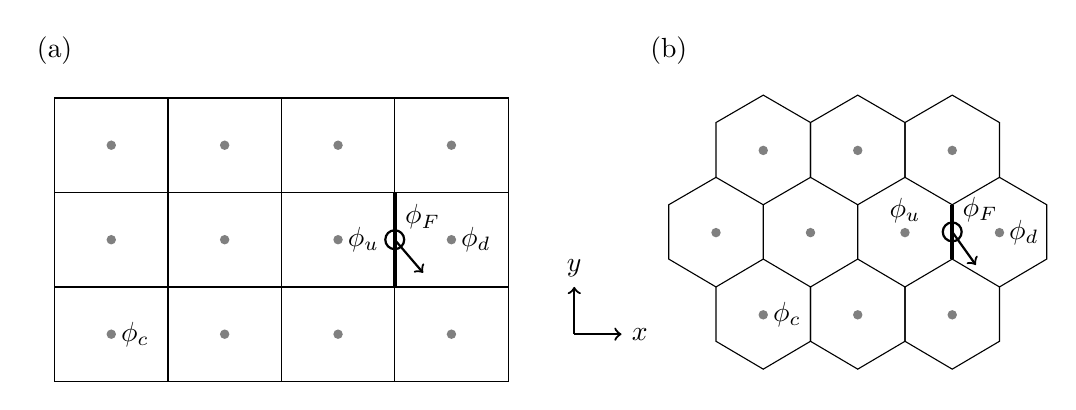
\begin{tikzpicture}[
  scale=0.6,
  cpnt/.style={fill=gray},
]

\begin{scope}[shift={(11,0)}]
	\draw [thick, ->] (0,1) -- (0,2) node [at end, anchor=south] {$y$};
	\draw [thick, ->] (0,1) -- (1,1) node [at end, anchor=west] {$x$};
\end{scope}

\node [above] at (0,6.5) {(a)};
\draw (0,0) rectangle (9.6,6);
\draw (0,2) -- (9.6,2);
\draw (0,4) -- (9.6,4);
\draw (0,0) -- (0,6);
\draw (2.4,0) -- (2.4,6);
\draw (4.8,0) -- (4.8,6);
\draw (7.2,0) -- (7.2,6);

\draw [ultra thick] (7.2,2) -- (7.2,4);
\draw [thick] (7.2,3) circle [radius=0.2] node [anchor=south west] {$\phi_F$};
\draw [thick, ->] (7.2,3) -- (7.8,2.3) node [anchor=west] {$\uf$};

\path [cpnt] (1.2,1) circle [radius=0.1] node [right] {$\phi_c$};
\path [cpnt] (1.2,3) circle [radius=0.1];
\path [cpnt] (1.2,5) circle [radius=0.1];

\path [cpnt] (3.6,1) circle [radius=0.1];
\path [cpnt] (3.6,3) circle [radius=0.1];
\path [cpnt] (3.6,5) circle [radius=0.1];

\path [cpnt] (6.0,1) circle [radius=0.1];
\path [cpnt] (6.0,3) circle [radius=0.1] node [right] {$\phi_u$};
\path [cpnt] (6.0,5) circle [radius=0.1];

\path [cpnt] (8.4,1) circle [radius=0.1];
\path [cpnt] (8.4,3) circle [radius=0.1] node [right] {$\phi_d$};
\path [cpnt] (8.4,5) circle [radius=0.1];

\begin{scope}[shift={(13,2)}]
	\node [above] at (0,4.5) {(b)};

	\draw (1,0) -- (0,0.59) -- (0,1.74) -- (1,2.32) -- (2,1.74) -- (2,0.59) -- (1,0); \path [cpnt] (1,1.15) circle [radius=0.1];
	\draw (2,1.74) -- (3,2.32) -- (4,1.74) -- (4,0.59) -- (3,0) -- (2,0.59); \path [cpnt] (3,1.15) circle [radius=0.1];
	\draw (4,1.74) -- (5,2.32) -- (6,1.74) -- (6,0.59) -- (5,0) -- (4,0.59); \path [cpnt] (5,1.15) circle [radius=0.1] node [above] {$\phi_u$};
	\draw (6,1.74) -- (7,2.32) -- (8,1.74) -- (8,0.59) -- (7,0) -- (6,0.59); \path [cpnt] (7,1.15) circle [radius=0.1] node [right] {$\phi_d$};

	\begin{scope}[shift={(1,-1.74)}]\draw (2,1.74) --(2,0.59) -- (1,0) -- (0,0.59) -- (0,1.74); \path [cpnt] (1,1.15) circle [radius=0.1] node [right] {$\phi_c$};\end{scope}
	\begin{scope}[shift={(3,-1.74)}]\draw (2,1.74) --(2,0.59) -- (1,0) -- (0,0.59) -- (0,1.74); \path [cpnt] (1,1.15) circle [radius=0.1];\end{scope}
	\begin{scope}[shift={(5,-1.74)}]\draw (2,1.74) --(2,0.59) -- (1,0) -- (0,0.59) -- (0,1.74); \path [cpnt] (1,1.15) circle [radius=0.1];\end{scope}

	\begin{scope}[shift={(1,1.74)}]\draw (0,0.59) -- (0,1.74) -- (1,2.32) -- (2,1.74) -- (2,0.59); \path [cpnt] (1,1.15) circle [radius=0.1];\end{scope}
	\begin{scope}[shift={(3,1.74)}]\draw (0,0.59) -- (0,1.74) -- (1,2.32) -- (2,1.74) -- (2,0.59); \path [cpnt] (1,1.15) circle [radius=0.1];\end{scope}
	\begin{scope}[shift={(5,1.74)}]\draw (0,0.59) -- (0,1.74) -- (1,2.32) -- (2,1.74) -- (2,0.59); \path [cpnt] (1,1.15) circle [radius=0.1];\end{scope}

	\draw [ultra thick] (6,0.59) -- (6,1.74);
	\draw [thick] (6,1.165) circle [radius=0.2] node [anchor=south west] {$\phi_F$};
	\draw [thick, ->] (6,1.165) -- (6.5,0.465) node [anchor=west] {$\uf$};
\end{scope}

\end{tikzpicture}
\end{document}

		\phantomsubcaption\label{fig:cubicFit:interiorStencils:quad}
		\phantomsubcaption\label{fig:cubicFit:interiorStencils:hex}
	\end{subfigure}
	\caption{Upwind-biased stencils for faces far away from the boundaries of two-dimensional
	(\subcaptionref{fig:cubicFit:interiorStencils:quad}) rectangular and
	(\subcaptionref{fig:cubicFit:interiorStencils:hex}) hexagon meshes.
	The stencil is used to fit a multidimensional polynomial to cell centre values, $\phi_c$, marked by grey circles, in order to approximate the value $\phi_F$ at the face centroid marked by an open circle.  $\phi_u$ and $\phi_d$ are the values at the centroids of the upwind and downwind cells neighbouring the target face, drawn with a heavy line.  The velocity vector $\uf$ is prescribed at face $f$ and determines the choice of stencil at each time-step.}
	\label{fig:cubicFit:interiorStencils}
\end{figure}

\TODO{cite previous work on cubicFit: \citep{lashley2002,thuburn2014,weller-shahrokhi2014}}
The cubicFit scheme approximates the value of the dependent variable at the face, $\phi_F$, using a least-squares fit over a stencil of surrounding known values.
To introduce the approximation method, we will consider how an approximate value is calculated for a face that is far away from the boundaries of a two-dimensional uniform rectangular mesh.
For any mesh, every interior face connects two adjacent cells.  The velocity direction at the face determines which of the two adjacent cells is the upwind cell.  Since the stencil is upwind-biased and asymmetric, two stencils must be constructed for every interior face, and the appropriate stencil is chosen depending on the velocity direction at each face for every time-step.

The upwind-biased stencil for a face $f$ is shown in figure~\ref{fig:cubicFit:interiorStencils:quad}.  The wind at the face, $\uf$, is blowing from the upwind cell $c_u$ to the downwind cell $c_d$.
To obtain an approximate value at $f$, a polynomial least-squares fit is calculated using the stencil values.
The stencil has \num{4} points in $x$ and \num{3} points in $y$, leading to a natural choice of polynomial that is cubic in $x$ and quadratic in $y$,
\begin{align}
	\phi = a_1 + a_2 x + a_3 y + a_4 x^2 + a_5 xy + a_6 y^2 + a_7 x^3 + a_8 x^2 y + a_9 x y^2 \label{eqn:cubicFit:fullPoly} \text{ .}
\end{align}
A least-squares approach is needed because the system of equations is overconstrained, with \num{12} stencil values but only \num{9} polynomial terms.  The stencil geometry is expressed in a local coordinate system with the face centroid as the origin so that the approximated value $\phi_F$ is equal to the constant coefficient $a_1$.
The stencil is upwind-biased to improve numerical stability, and the multidimensional cubic polynomial is chosen to improve accuracy in the direction of flow \citep{leonard1993}.

The remainder of this section generalises the approximation technique for arbitrary meshes and describes the methods for constructing stencils, performing a least-squares fit with a suitable polynomial, and ensuring numerical stability of the transport scheme.

\subsubsection{Stencil construction}
\label{sec:cubicFit:stencil}

For every interior face, two stencils are constructed, one for each of the possible upwind cells.
Stencils are not constructed for boundary faces because values of $\phi$ at boundaries are calculated from prescribed boundary conditions.
For a given interior face $f$ and upwind cell $c_u$, we find those faces that are connected to $c_u$ and `oppose' face $f$.  These are called the \textit{opposing faces}.
The opposing faces for face $f$ and upwind cell $c_u$ are determined as follows.
Defining $G$ to be the set of faces other than $f$ that border cell $c_u$, we calculate the `opposedness', $\Opp$, between faces $f$ and $g \in G$, defined as
\begin{align}
	\Opp(f, g) \equiv - \frac{\Sf \cdot \vect{S}_g}{\magSf^2} \label{eqn:cubicFit:opp}
\end{align}
where $\Sf$ and $\vect{S}_g$ are the surface area vectors pointing outward from cell $c_u$ for faces $f$ and $g$ respectively.
Using the fact that $\vect{a} \cdot \vect{b} = \Mag{\vect{a}}\:\Mag{\vect{b}} \cos(\theta)$ we can rewrite equation~\eqref{eqn:cubicFit:opp} as
\begin{align}
	\Opp(f, g) = - \frac{\Mag{\vect{S}_g}}{\magSf} \cos(\theta)
\end{align}
where $\theta$ is the angle between faces $f$ and $g$.  In this form, it can be seen that $\Opp$ is a measure of the relative area of $g$ and how closely it parallels face $f$.

The set of opposing faces, $\mathrm{OF}$, is a subset of $G$, comprising those faces with $\Opp \geq 0.5$, and the face with the maximum opposedness.  Expressed in set notation, this is
\begin{align}
	\mathrm{OF}(f,c_u) \equiv \{ g : \Opp(f, g) \geq 0.5 \} \cup \{ g : \max_{g\:\in\:G}(\Opp(f, g)) \} \text{ .}
\end{align}
On a rectangular mesh, there is always one opposing face $g$, and it is exactly parallel to the face $f$ such that $\Opp(f, g) = 1$.

Once the opposing faces have been determined, the set of internal and external cells must be found.  The \textit{internal cells} are those cells that are connected to the opposing faces.  Note that $c_u$ is always an internal cell.  The \textit{external cells} are those cells that share vertices with the internal cells.  Note that $c_d$ is always an external cell.  Finally, the \textit{stencil boundary faces} are boundary faces having Dirichlet boundary conditions\footnote{Boundary faces with Neumann boundary conditions would require extrapolated boundary values to be calculated.
This would create a feedback loop in which boundary values are extrapolated from interior values, then interior values are transported using stencils that include boundary values.  
We have not considered how such an extrapolation could be made consistent with the multidimensional polynomial reconstruction.
Hence, boundary faces with Neumann boundary conditions are excluded from the set of stencil boundary faces.} that share a vertex with the internal cells.
Having found these three sets, the stencil is constructed to comprise all internal cells, external cells and stencil boundary faces.

\begin{figure}
	\centering
	\documentclass[tikz]{standalone}
\newcommand{\iu}{{i\mkern1mu}}
\newcommand{\vect}{\mathbf}
\newcommand{\unitg}{\vect{\hat{g}}}
\newcommand{\unitn}{\vect{\hat{n}}}
\newcommand{\uf}{\vect{u}_f}
\newcommand{\Opp}{\mathrm{Opp}}
\newcommand{\Sf}{\vect{S}_f}
\newcommand{\Mag}[1]{\lvert #1 \rvert}
\newcommand{\magSf}{\Mag{\Sf}}
\newcommand{\area}{\mathcal{A}}
\newcommand{\vol}{\mathcal{V}}
\newcommand{\volave}[1]{\langle #1 \rangle_\vol}
\newcommand{\moment}{\mathfrak{m}}
\newcommand{\rhoexp}{\mathfrak{n}}

\usetikzlibrary{plotmarks}
\usetikzlibrary{patterns}
\begin{document}
\begin{tikzpicture}[
  scale=0.25,
  cpnt/.style={fill=black},
]
\fill [pattern=north east lines,pattern color=gray] (5,0) -- (6,4) -- (3,7) -- (5, 15) -- (7,19) -- (1,19) -- (1,0);
\node at (0,9.5) {\rotatebox{90}{Dirichlet boundary}};

\draw [white] (-1,-2.1) rectangle (-1,-2);
\draw [thick, ->] (-1,-1.5) -- (4,-1.5) node [midway, anchor=south] {$\vect{u}$};

\draw [thick, ->] (20.7,7.5) -- (19.7,10) node [at end, anchor=south] {$y$};
\draw [thick, ->] (20.7,7.5) -- (23.1,8.35) node [at end, anchor=north] {$x$};

\draw (10,5) -- (20,7) -- (18,12) -- (11,14);
\draw [densely dashed, ultra thick] (11,14) -- (7,8) -- (10,5);
\draw [ultra thick] (20,7) -- (18,12);
\draw [thick] (19,9.5) circle [radius=0.35] node [anchor=east] {$f$};
\path [cpnt] (13.3,9.5) circle [radius=0.4] node [anchor=west, black] {$c_u$};
\path [fill=gray] (21.7,9.5) circle [radius=0.4] node [anchor=west, black] {$c_d$};

% direct upwind cells
\draw (10,5) -- (6,4) -- (3,7) -- (7,8);
\path [cpnt] (6.5,6) circle [radius=0.4];

\draw (3,7) -- (5,15) -- (11,14);
\path [cpnt] (6.3,11) circle [radius=0.4];

\draw (20,7) -- (24,6) -- (25,13) -- (18,12);
\draw (20,7) -- (19,3) -- (25,2) -- (24,6);
\draw (19,3) -- (11,1) -- (10,5);
\draw (11,14) -- (12,18) -- (16,18) -- (18,12);
\draw (16,18) -- (21,19) -- (25,13);
\draw (5,15) -- (7,19) -- (12,18);
\draw (6,4) -- (5,0) -- (11,1);

% vertices
\node at (3,7) {\pgfuseplotmark{square*}};
\node at (5,15) {\pgfuseplotmark{square*}};
\node at (11,14) {\pgfuseplotmark{square*}};
\node at (18,12) {\pgfuseplotmark{square*}};
\node at (10,5) {\pgfuseplotmark{square*}};
\node at (20,7) {\pgfuseplotmark{square*}};
\node at (6,4) {\pgfuseplotmark{square*}};
\node at (7,8) {\pgfuseplotmark{square*}};
\node at (5.5,2) [scale=1.5,rotate=60] {\pgfuseplotmark{triangle*}};
\node at (6,17) [scale=1.5,rotate=60] {\pgfuseplotmark{triangle*}};
\node at (4,11) [scale=1.5,rotate=60] {\pgfuseplotmark{triangle*}};
\node at (4.5,5.5) [scale=1.5,rotate=60] {\pgfuseplotmark{triangle*}};
\end{tikzpicture}
\end{document}

%	\includegraphics{../fig-double-upwind-stencil/fig-double-upwind-stencil.pdf}
	%
	\caption{A fourteen-point, upwind-biased stencil for face $f$ connecting the pentagonal upwind cell, $c_u$, and the downwind cell $c_d$.  The dashed lines denote the two faces of cell $c_u$ that oppose $f$, and black circles mark the centroids of the internal cells that are connected to these two opposing faces.  The stencil is extended outwards by including cells that share vertices with the three internal cells, where black squares mark these vertices.  Four stencil boundary faces, marked by black triangles, are also included.
The local coordinate system $(x, y)$ has its origin at the centroid of face $f$, marked by an open circle, with $x$ normal to $f$ and $y$ perpendicular to $x$.}
	\label{fig:double-upwind-stencil}
\end{figure}

Figure~\ref{fig:double-upwind-stencil} illustrates a stencil construction for face $f$ connecting upwind cell $c_u$ and downwind cell $c_d$.  The two opposing faces are denoted by thick dashed lines and the centres of the three adjoining internal cells are marked by black circles.  The stencil is extended outwards by including the external cells that share vertices with the internal cells, where the vertices are marked by black squares.  A boundary at the far left has Dirichlet boundary conditions, and so the four stencil boundary faces are also included in the stencil, where the boundary face centres are marked by black triangles.  The resultant stencil contains fourteen points.

\subsubsection{Least-squares fit}
To approximate the value of $\phi$ at a face $f$, a least-squares fit is calculated from a stencil of surrounding known values.  First, we will show how a polynomial least-squares fit is calculated for a face on a rectangular mesh.  Second, we will make modifications to the least-squares fit that are necessary for numerical stability.  

For faces that are far away from the boundaries of a rectangular mesh, we fit the multidimensional polynomial given by equation~\eqref{eqn:cubicFit:fullPoly} that has nine unknown coefficients, $\vect{a} = a_1 \ldots a_9$, using the twelve cell centre values from the upwind-biased stencil, $\bm{\phi} = \phi_1 \ldots \phi_{12}$.  This yields a matrix equation
\begin{align}
	\begin{bmatrix}
		1 & x_1 & y_1 & x_1^2 & x_1 y_1 & y_1^2 & x_1^3 & x_1^2 y_1 & x_1 y_1^2 \\
		1 & x_2 & y_2 & x_2^2 & x_2 y_2 & y_2^2 & x_2^3 & x_2^2 y_2 & x_2 y_2^2 \\
		\vdots & \vdots & \vdots & \vdots & \vdots & \vdots & \vdots & \vdots & \vdots \\
		1 & x_{12} & y_{12} & x_{12}^2 & x_{12} y_{12} & y_{12}^2 & x_{12}^3 & x_{12}^2 y_{12} & x_{12} y_{12}^2 \\
	\end{bmatrix}
	\begin{bmatrix}
		a_1 \\
		a_2 \\
		\vdots \\
		a_9
	\end{bmatrix}
	=
	\begin{bmatrix}
		\phi_1 \\
		\phi_2 \\
		\vdots \\
		\phi_{12}
	\end{bmatrix}
\end{align}
which can be written as
\begin{align}
	\vect{B} \vect{a} = \bm{\phi} \label{eqn:cubicFit:unweightedLeastSquares} \text{ .}
\end{align}
The rectangular matrix $\vect{B}$ has one row for each cell in the stencil and one column for each term in the polynomial.  $\vect{B}$ is called the \textit{stencil matrix}, and it is constructed using only the mesh geometry.
A local coordinate system is established in which $x$ is normal to the face $f$ and $y$ is perpendicular to $x$.
The coordinates $(x_i, y_i)$ give the position of the centroid of the $i$th cell in the stencil.
A two-dimensional stencil is also used for the tests on spherical meshes in section~\ref{sec:cubicFit:deformationSphere}.  In these tests, cell centres are projected perpendicular to a tangent plane at the face centre.  Previous studies found that results were largely insensitive to the projection method \citep{skamarock-gassmann2011,lashley2002}.

The unknown coefficients $\vect{a}$ are calculated using the pseudo-inverse, $\vect{B}^+$, found by singular value decomposition,
\begin{align}
	\vect{a} = \vect{B}^+ \bm{\phi} \text{ .}
%
\intertext{Recall that the approximate value $\phi_F$ is equal to the constant coefficient $a_1$, which is a weighted mean of $\bm{\phi}$,} 
%
	a_1 = \begin{bmatrix}
		b_{1,1}^+ \\
		b_{1,2}^+ \\
		\vdots \\
		b_{1,12}^+
	\end{bmatrix}
	\cdot
	\begin{bmatrix}
		\phi_1 \\
		\phi_2 \\
		\vdots \\
		\phi_{12}
	\end{bmatrix} \label{eqn:cubicFit:weighted-sum}
\end{align}
where the weights $b_{1,1}^+ \ldots b_{1,12}^+$ are the elements of the first row of $\vect{B}^+$.
Note that the majority of the least-squares fit procedure depends on the mesh geometry only.  An implementation may precompute the pseudo-inverse for each stencil during model initialisation, and only the first row needs to be stored.  Since each face has two possible stencils depending on the orientation of the velocity relative to the face, the implementation stores two sets of weights for each face.
Knowledge of the values of $\bm{\phi}$ is only required to calculate the weighted mean given by equation~\eqref{eqn:cubicFit:weighted-sum}, which is evaluated once per face per time-stage.

In the least-squares fit presented above, all stencil values contributed equally to the polynomial fit.
It is necessary for numerical stability that the polynomial fits the cells connected to face $f$ more closely than other cells in the stencil, as shown by \citet{lashley2002,skamarock-menchaca2010}.
To achieve this, we allow each cell to make an unequal contribution to the least-squares fit.
We assign an integer \textit{multiplier} to each cell in the stencil, $\vect{m} = m_1 \ldots m_{12}$, and multiply equation~\eqref{eqn:cubicFit:unweightedLeastSquares} to obtain
\begin{align}
	\vect{\tilde{B}} \vect{a} = \vect{m} \cdot \bm{\phi}
\end{align}
where $\vect{\tilde{B}} = \vect{M} \vect{B}$ and $\vect{M} = \mathrm{diag}(\vect{m})$.  The constant coefficient $a_1$ is calculated from the pseudo-inverse, $\vect{\tilde{B}}^+$,
\begin{align}
	a_1 = \vect{\tilde{b}_1^+} \cdot \vect{m} \cdot \bm{\phi} \label{eqn:cubicFit:weightedPinv}
\end{align}
where $\vect{\tilde{b}_1^+} = \tilde{b}_{1,1}^+ \ldots \tilde{b}_{1,12}^+$ are the elements of the first row of $\vect{\tilde{B}}^+$.
Again, $a_1$ is a weighted mean of $\bm{\phi}$, where the weights are now $\vect{\tilde{b}_1^+} \cdot \vect{m}$.  Values for $\vect{m}$ are chosen so that the cells connected to face $f$ make a greater contribution to the least-squares fit, as discussed later in section~\ref{sec:cubicFit:stabilisation}.

For faces of a non-rectangular mesh, or faces that are near a boundary, the number of stencil points and number of polynomial terms may differ: a stencil will have one or more cells and, for two-dimensional meshes, its polynomial will have between one and nine terms.  Additionally, the polynomial cannot have more terms than its stencil has cells because this would lead to an underconstrained system of equations.  The procedure for choosing suitable polynomials is discussed next.

\subsubsection{Polynomial generation}
\label{sec:cubicFit:polyGen}

\begin{figure}
	\centering
	\begin{subfigure}{\textwidth}
		\centering
		\documentclass[tikz]{standalone}
\newcommand{\iu}{{i\mkern1mu}}
\newcommand{\vect}{\mathbf}
\newcommand{\unitg}{\vect{\hat{g}}}
\newcommand{\unitn}{\vect{\hat{n}}}
\newcommand{\uf}{\vect{u}_f}
\newcommand{\Opp}{\mathrm{Opp}}
\newcommand{\Sf}{\vect{S}_f}
\newcommand{\Mag}[1]{\lvert #1 \rvert}
\newcommand{\magSf}{\Mag{\Sf}}
\newcommand{\area}{\mathcal{A}}
\newcommand{\vol}{\mathcal{V}}
\newcommand{\volave}[1]{\langle #1 \rangle_\vol}
\newcommand{\moment}{\mathfrak{m}}
\newcommand{\rhoexp}{\mathfrak{n}}

\usetikzlibrary{patterns}
\begin{document}
\begin{tikzpicture}[
  scale=0.65,
  cpnt/.style={fill=gray},
]

\node [above] at (0,6) {(a)};
\fill [pattern=north east lines,pattern color=gray] (0,-1) rectangle (9,0);
\node at (4.5,-1.5) {Lower boundary};
\draw (0,0) rectangle (9,4);
\draw (3,0) -- (3,4);
\draw (6,0) -- (6,4);
\draw (0,2) -- (9,2);

\draw [ultra thick] (3,2) -- (6,2);
\draw [thick] (4.5,2) circle [radius=0.2];

\path [cpnt] (1.5,1) circle [radius=0.1];
\path [cpnt] (4.5,1) circle [radius=0.1] node [right] {$\phi_u$};
\path [cpnt] (7.5,1) circle [radius=0.1];
\path [cpnt] (1.5,3) circle [radius=0.1];
\path [cpnt] (4.5,3) circle [radius=0.1] node [right] {$\phi_d$};
\path [cpnt] (7.5,3) circle [radius=0.1];
\draw [thick, ->] (4.5,2) -- (5,2.35) node [anchor=west] {$\uf$};

\draw [<->] (6,5) node [left] {$y$} -- (7,5) -- (7,6) node [above] {$x$};

\begin{scope}[shift={(10,0)}]
\node [above] at (0,6) {(b)};
\fill [pattern=north east lines,pattern color=gray] (0,-1) rectangle (9,0);
\node at (4.5,-1.5) {Lower boundary};
\draw (0,0) rectangle (9,6);
\draw (3,0) -- (3,6);
\draw (6,0) -- (6,6);
\draw (0,2) -- (9,2);
\draw (0,4) -- (9,4);

\draw [ultra thick] (3,4) -- (6,4);
\draw [thick] (4.5,4) circle [radius=0.2];

\path [cpnt] (1.5,1) circle [radius=0.1];
\path [cpnt] (4.5,1) circle [radius=0.1];
\path [cpnt] (7.5,1) circle [radius=0.1];
\path [cpnt] (1.5,3) circle [radius=0.1];
\path [cpnt] (4.5,3) circle [radius=0.1] node [right] {$\phi_u$};
\path [cpnt] (7.5,3) circle [radius=0.1];
\path [cpnt] (1.5,5) circle [radius=0.1];
\path [cpnt] (4.5,5) circle [radius=0.1] node [right] {$\phi_d$};
\path [cpnt] (7.5,5) circle [radius=0.1];
\draw [thick, ->] (4.5,4) -- (5,4.35) node [anchor=west] {$\uf$};

\draw [<->] (10,5) node [left] {$y$} -- (11,5) -- (11,6) node [above] {$x$};
\end{scope}

\end{tikzpicture}
\end{document}

		\phantomsubcaption\label{fig:cubicFit:boundaryStencils:two}
		\phantomsubcaption\label{fig:cubicFit:boundaryStencils:three}
	\end{subfigure}
	\caption{Upwind-biased stencils for faces near the lower boundary of a rectangular $x$--$z$ mesh, with
	(\subcaptionref{fig:cubicFit:boundaryStencils:two}) a $3 \times 2$ stencil for the face immediately adjacent to the lower boundary, and
	(\subcaptionref{fig:cubicFit:boundaryStencils:three}) a $3 \times 3$ stencil for the face immediately adjacent to the face in (\subcaptionref{fig:cubicFit:boundaryStencils:two}).  Each stencil belongs to the face marked by a thick line.  The local coordinate system is shown, having an $x$ direction normal to the face a $y$ direction tangent to the face.  For both stencils, attempting a least-squares fit using the nine-term polynomial in equation~\eqref{eqn:cubicFit:fullPoly} would result in an underconstrained problem.
	There is no normal flow at the lower boundary.}
	\label{fig:cubicFit:boundaryStencils}
\end{figure}

The majority of faces on a uniform two-dimensional mesh have stencils with more than nine cells.  For example, a rectangular mesh has 12 points (figure~\ref{fig:cubicFit:interiorStencils:quad}), and a hexagonal mesh has 10 points (figure~\ref{fig:cubicFit:interiorStencils:hex}).
In both cases, constructing a system of equations using the nine-term polynomial in equation~\eqref{eqn:cubicFit:fullPoly} leads to an overconstrained problem that can be solved using least-squares.
However, this is not true for faces near boundaries: stencils that have fewer than nine cells (figure~\ref{fig:cubicFit:boundaryStencils:two}) would result in an underconstrained problem, and stencils that have exactly nine cells may lack sufficient information to constrain high-order terms.
For example, the stencil in figure~\ref{fig:cubicFit:boundaryStencils:three} lacks sufficient information to fit the $x^3$ term.  In such cases, it becomes necessary to perform a least-squares fit using a polynomial with fewer terms.

For every stencil, we find a set of \textit{candidate polynomials} that do not result in an underconstrained problem.
In two dimensions, a candidate polynomial has some combination of between one and nine terms from equation~\eqref{eqn:cubicFit:fullPoly}.  There are two additional constraints that a candidate polynomial must satisfy.

First, high-order terms may be included in a candidate polynomial only if the lower-order terms are also included.
More precisely, let
\begin{align}
	M(x, y) = { x^i y^j : i,j \geq 0 \text{ and } i \leq 3 \text{ and } j \leq 2 \text{ and } i+j \leq 3}
\end{align}
be the set of all monomials of degree at most \num{3} in $x, y$.
A subset $S$ of $M(x,y)$ is ``dense'' if, whenever $x^a y^b$ is in $S$, then $x^i y^j$ is also in $S$ for all $0 \leq i \leq a$, $0 \leq j \leq b$.
For example, the polynomial $\phi = a_1 + a_2 x + a_3 y + a_4 xy + a_5 x^2 + a_6 x^2 y$ is a dense subset of $M(x,y)$, but $\phi = a_1 + a_2 x + a_3 y + a_4 x^2 y$ is not because $x^2 y$ can be included only if $xy$ and $x^2$ are also included.
In total there are 26 dense subsets of the two-dimensional polynomial in equation~\eqref{eqn:cubicFit:fullPoly}.

Second, a candidate polynomial must have a stencil matrix $\vect{B}$ that is full rank.  The matrix is considered full rank if its smallest singular value is greater than \num{1e-9}.
Using a polynomial with all nine terms and the stencil in figure~\ref{fig:cubicFit:boundaryStencils:three} results in a rank-deficient matrix and so the nine-term polynomial is not a candidate polynomial.

The candidate polynomials are all the dense subsets of $M(x,y)$ that have a cardinality greater than one with a stencil matrix that is full rank.  The final stage of the cubicFit transport scheme selects a candidate polynomial and ensures that the least-squares fit is numerically stable.

\subsubsection{Achieving numerical stability}
\label{sec:cubicFit:stabilisation}
So far, we have constructed a stencil and found a set of candidate polynomials.  Applying a least-squares fit to any of these candidate polynomials avoids creating an underconstrained problem.  The final stage of the transport scheme chooses a suitable candidate polynomial and appropriate multipliers $\vect{m}$ so that the fit is numerically stable.

The approximated value $\phi_F$ is equal to $a_1$ which is calculated from equation~\eqref{eqn:cubicFit:weightedPinv}.  The value of $a_1$ is a weighted mean of $\bm{\phi}$ where $\vect{w} = \vect{\tilde{b}_1^+} \cdot \vect{m}$ are the weights.
If the cell centre values $\bm{\phi}$ are assumed to approximate a smooth field then we expect $\phi_F$ to be close to the values of $\phi_u$ and $\phi_d$, and expect $\phi_F$ to be insensitive to small changes in $\bm{\phi}$.
When the weights $\vect{w}$ have large magnitude then this is no longer true: $\phi_F$ becomes sensitive to small changes in $\bm{\phi}$ which can result in large, numerically unstable departures from the smooth field $\bm{\phi}$.

To avoid numerical instabilities, simplified, one-dimensional von Neumann analyses were performed in order to impose stability conditions on the weights $\vect{w}$.
The first analysis uses a two-cell approximation to derive separate stability conditions involving the upwind weight $w_u$ and downwind weight $w_d$.  The second analysis uses three cells to derive a stability condition that involves all weights in a stencil.

The two-cell analysis starts with the conservation equation for a dependent variable $\phi$ that is discrete-in-space and continuous-in-time
\begin{align}
\frac{\partial \phi_j}{\partial t} &= - v \frac{\phi_R - \phi_L}{\Delta x} \label{eqn:vonNeumann:advectionLR} \\
%
\intertext{where $v$ is the velocity, and the left and right fluxes, $\phi_L$ and $\phi_R$, are weighted averages of the neighbouring cell centres.  Assuming that $v$ is positive}
%
\phi_L &= \alpha_u \phi_{j-1} + \alpha_d \phi_j \\
\phi_R &= \beta_u \phi_j + \beta_d \phi_{j+1}
\end{align}
where $\phi_{j-1}, \phi_j, \phi_{j+1}$ are cell centre values, and $j$ denotes a cell centre position $x = j \Delta x$ where $\Delta x$ is a uniform mesh spacing.
$\alpha_u$ and $\beta_u$ are the upwind weights and $\alpha_d$ and $\beta_d$ are the downwind weights for the left and right fluxes respectively, and $\alpha_u + \alpha_d = 1$ and $\beta_u + \beta_d = 1$.

At a given time $t = n \Delta t$ at time-level $n$ and with a time-step $\Delta t$, we assume a wave-like solution with an amplification factor $A$, such that
\begin{align}
	\phi_j^{(n)} &= A^n e^{\iu j k \Delta x} \label{eqn:vonNeumann:fourier}
\end{align}
where $\phi_j^{(n)}$ denotes a value of $\phi$ at position $j$ and time-level $n$.  Using this to rewrite the left-hand side of equation~\eqref{eqn:vonNeumann:advectionLR}
\begin{align}
\frac{\partial \phi_j}{\partial t} &= \frac{\partial}{\partial t} \left( A^{t / \Delta t} \right) e^{ijk\Delta x} = \frac{\ln A}{\Delta t} A^n e^{ikj\Delta x} \\
%
\shortintertext{hence equation~\eqref{eqn:vonNeumann:advectionLR} becomes}
%
\frac{\ln A}{\Delta t} &= - \frac{v}{\Delta x} \left( \beta_u + \beta_d e^{ik\Delta x} - \alpha_u e^{-ik\Delta x} - \alpha_d \right) \\
\ln A &= -c \left( \beta_u - \alpha_d + \beta_d \cos k\Delta x + \iu \beta_d \sin k \Delta x - \alpha_u \cos k\Delta x + \iu \alpha_u \sin k\Delta x \right)
%
\intertext{where the Courant number $c = v \Delta t / \Delta x$.
Let $\Re = \beta_u - \alpha_d + \beta_d \cos k\Delta x - \alpha_u \cos k\Delta x$ and
$\Im = \beta_d \sin k \Delta x + \alpha_u \sin k\Delta x$, then}
%
\ln A &= -c \left( \Re + \iu \Im \right) \\
A &= e^{-c \Re} e^{-\iu c \Im} \\
%
\shortintertext{and the complex modulus of $A$ is}
%
|A| &= e^{-c \Re} = \exp \left( -c \left( \beta_u - \alpha_d + \left(\beta_d - \alpha_u \right) \cos k\Delta x \right) \right) \text{ .}
\end{align}
For stability we need $|A| \leq 1$ and, imposing the additional constraints that $\alpha_u = \beta_u$ and $\alpha_d = \beta_d$, then
\begin{align}
\left( \alpha_u - \alpha_d \right) \left( 1 - \cos k\Delta x \right) &\geq 0 \quad \forall k\Delta x
%
\shortintertext{and, given $0 \leq 1 - \cos k \Delta x \leq 2$, then}
%
\alpha_u - \alpha_d \geq 0 \text{ .} \label{eqn:vonNeumann:twopoint-lower}
\end{align}
Additionally, we do not want more damping than a first-order upwind scheme (where $\alpha_u = \beta_u = 1$, $\alpha_d = \beta_d = 0$), having an amplification factor, $A_\mathrm{up}$, so we need $\left\lvert A \right\rvert \geq \left\lvert A_\mathrm{up} \right\rvert$, hence
\begin{align}
	\exp \left( -c \left(\alpha_u - \alpha_d\right) \left( 1 - \cos k\Delta x \right) \right) &\geq \exp \left( -c \left(1 - \cos k\Delta x \right) \right) \quad \forall k\Delta x
%
\shortintertext{therefore}
%
	\alpha_u - \alpha_d &\leq 1 \text{ .} \label{eqn:vonNeumann:twopoint-upper}
\end{align}
Now, knowing that $\alpha_u + \alpha_d = 1$ (or $\alpha_d = 1 - \alpha_u$) then, using equations~\eqref{eqn:vonNeumann:twopoint-lower} and \eqref{eqn:vonNeumann:twopoint-upper}, we obtain the first two stability conditions,
\begin{align}
	0.5 \leq \alpha_u &\leq 1 \text{ and} \label{eqn:vonNeumann:upwind} \\
	0 \leq \alpha_d &\leq 0.5 \label{eqn:vonNeumann:downwind} \text{ .}
\end{align}

The three-cell analysis starts again from equation~\eqref{eqn:vonNeumann:advectionLR} but this time approximate $\phi_L$ and $\phi_R$ using three cell centre values,
\begin{align}
	\phi_L &= \alpha_{uu} \phi_{j-2} + \alpha_u \phi_{j-1} + \alpha_d \phi_j \\
	\phi_R &= \alpha_{uu} \phi_{j-1} + \alpha_u \phi_j + \alpha_d \phi_{j+1}
\end{align}
having used the same weights $\alpha_{uu}$, $\alpha_u$ and $\alpha_d$ for both left and right fluxes.
Substituting equation~\eqref{eqn:vonNeumann:fourier} into equation~\eqref{eqn:vonNeumann:advectionLR} we find
\begin{align}
A = \exp\left( -c \left[ \alpha_{uu} \left( e^{-ik\Delta x} - e^{-2ik\Delta x} \right) + \alpha_u \left( 1 - e^{-ik\Delta x} \right) + \alpha_d \left( e^{ik\Delta x} - 1 \right) \right] \right)
%
\intertext{so that, if the complex modulus $\left\lvert A \right\rvert \leq 1$ then}
%
\alpha_u - \alpha_d + \left( \alpha_{uu} - \alpha_u + \alpha_d \right) \cos k\Delta x - \alpha_{uu} \cos 2k\Delta x \geq 0 \text{ .}
\end{align}
If $k\Delta x = \pi$ then $\cos k\Delta x = -1$ and $\cos 2k\Delta x = 1$ and $\alpha_u - \alpha_d \geq \alpha_{uu}$.  If $k\Delta x = \pi / 2$ then $\cos k\Delta x = 0$ and $\cos 2k\Delta x = -1$ and $\alpha_u - \alpha_d \geq -\alpha_{uu}$.  Hence we find that
\begin{align}
	\alpha_u - \alpha_d &\geq \left\lvert\alpha_{uu}\right\rvert \label{eqn:vonNeumann:uuConstraint} \text{ .}
%
	\intertext{When the same analysis is performed with four cells, $\alpha_{uuu}$, $\alpha_{uu}$, $\alpha_u$ and $\alpha_d$, by varying $k \Delta x$ we find that equation~\eqref{eqn:vonNeumann:uuConstraint} holds replacing $\left\lvert \alpha_{uu} \right\rvert$ with $\max(\left\lvert\alpha_{uu}\right\rvert, \left\lvert\alpha_{uuu}\right\rvert)$.  Hence, we generalise equation~\eqref{eqn:vonNeumann:uuConstraint} to obtain the final stability condition}
%
	\alpha_u - \alpha_d &\geq \max_{p\:\in\:P} |\alpha_p|
\end{align}
where the peripheral cells $P$ is the set of all stencil cells except for the upwind cell and downwind cell, and $\alpha_p$ is the weight for a given peripheral cell $p$.
The three stability conditions (equations~\ref{eqn:vonNeumann:upwind}, \ref{eqn:vonNeumann:downwind} and \ref{eqn:vonNeumann:uuConstraint}) are used to impose three stability conditions on the weights $\vect{w}$,
\begin{subequations}
\label{eqn:cubicFit:stability}
\begin{align}
	0.5 \leq w_u \leq 1 \label{eqn:cubicFit:stabilityU} \\
	0 \leq w_d \leq 0.5 \label{eqn:cubicFit:stabilityD} \\
	w_u - w_d \geq \max_{p\:\in\:P}(|w_p|)
\end{align}
\end{subequations}
where $w_u$ and $w_d$ are the weights for the upwind and downwind cells respectively.  The \textit{peripheral points} $P$ are the cells in the stencil that are not the upwind or downwind cells, and $w_p$ is the weight for a given peripheral point $p$.
 The upwind, downwind and peripheral weights sum to one such that $w_u + w_d + \sum_{p \in P} w_p = 1$.
We hypothesise that the stability conditions given by equation~\eqref{eqn:cubicFit:stability} are necessary but not sufficient for a transport scheme on arbitrary meshes.

The stability of the one-dimensional transport equation discretised in space and time could be analysed using existing techniques \citep{baldauf2008}, but we have only analysed the spatial stability of the cubicFit scheme.  Numerical experiments presented in section~\ref{sec:slanted:mountainAdvect} demonstrate that the cubicFit scheme is generally insensitive to the time-step, provided that it is below a stability limit.

\subsubsection{Stabilisation procedure}

Equipped with three stability conditions in equation~\ref{eqn:cubicFit:stability}, we develop a stabilisation procedure that achieves numerical stability on arbitrary meshes.
The stabilisation procedure comprises three steps.  In the first step, the set of candidate polynomials is sorted in preference order so that candidates with more terms are preferred over those with fewer terms.
If there are multiple candidates with the same number of terms, the minimum singular value of $\vect{B}$ is calculated for each candidate, and an ordering is imposed such that the candidate with the larger minimum singular value is preferred.  This ordering ensures that the preferred candidate is the highest-order polynomial with the most information content.\footnote{Note that singular values are used for two purposes: first, to test if the matrix $\vect{B}$ is full-rank and, second, to impose an ordering on candidates.
We have used the minimum singular value, $\sigma_\mathrm{min}(\vect{B})$, for both purposes.  Alternatively, we could use the condition number, $\mathrm{cond}(\vect{B})$, which is the ratio of smallest to largest singular value.
Experiments revealed that only the candidate ordering was sensitive to the choice of $\sigma_\mathrm{min}$ or $\mathrm{cond}$.
The most suitable choices of singular value calculations could be explored in future.}

In the second step, the most-preferred polynomial is taken from the list of candidates and the multipliers are assigned so that the upwind cell and downwind cell have multipliers $m_u = 2^{10}$ and $m_d = 2^{10}$ respectively, and all peripheral points have multipliers $m_p = 1$.  These multipliers are very similar to those used by \citet{lashley2002}, leading to a well-conditioned matrix $\vect{\tilde{B}}$ and a least-squares fit in which the polynomial passes almost exactly through the upwind and downwind cell centre values.

In the third step, we calculate the weights $\vect{w}$ and evaluate them against the stability conditions given in equation~\eqref{eqn:cubicFit:stability}.
If any condition is violated, the value of $m_d$ is halved and the conditions are evaluated with the new weights.  This step is repeated until the weights satisfy the stability conditions, or $m_d$ becomes smaller than one.  In practice, the conditions are satisified when $m_d$ is either small (between 1 and 4) or equal to $2^{10}$.  The upwind multiplier $m_u$ is fixed at $2^{10}$ and the peripheral multipliers $m_p$ are fixed at \num{1}.  If the conditions are still not satisfied, then we start again from the second step with the next polynomial in the candidate list. 

Finally, if no stable weights are found for any candidate polynomial, we revert to an upwind scheme such that $w_u = 1$ and all other weights are zero.
In our experiments we have not encountered any stencil for which this last resort is required.
Furthermore, our experiments show that the stabilisation procedure only modifies the least squares fit for stencils near boundaries and for stencils in distorted mesh regions.
For stencils in the interior of a uniform rectangular mesh, the least squares fit includes all terms in equation~\eqref{eqn:cubicFit:fullPoly} with $m_u = m_d = 2^{10}$.

\begin{figure}
	\centering
	\begin{subfigure}{\textwidth}
		\centering
		\input{cubicFit/stabilisation}
		\phantomsubcaption\label{fig:cubicFit:oscillatory1D:cubic}
		\phantomsubcaption\label{fig:cubicFit:oscillatory1D:quadratic}
		\phantomsubcaption\label{fig:cubicFit:oscillatory1D:quadraticUpwind}
	\end{subfigure}
	\caption{One-dimensional least-squares fits with a stencil of five points using
	(\subcaptionref{fig:cubicFit:oscillatory1D:cubic}) a cubic polynomial with multipliers $m_u = 1024$, $m_d = 1024$ and $m_p = 1$,
	(\subcaptionref{fig:cubicFit:oscillatory1D:quadratic}) a quadratic polynomial with the same multipliers, and
	(\subcaptionref{fig:cubicFit:oscillatory1D:quadraticUpwind}) a quadratic polynomial with multipliers $m_u = 1024$, $m_d = 1$ and $m_p = 1$.
	Notice that the curves in
	(\subcaptionref{fig:cubicFit:oscillatory1D:cubic}) and
	(\subcaptionref{fig:cubicFit:oscillatory1D:quadratic}) fit almost exactly through the upwind and downwind points immediately adjacent to the $y$-axis, but in
	(\subcaptionref{fig:cubicFit:oscillatory1D:quadraticUpwind}) the curve fits almost exactly only through the upwind point immediately to the left of the $y$-axis.  The point data are labelled with their respective weights.
	Points that have failed one of the stability conditions in equation~\eqref{eqn:cubicFit:stability} are marked in red with italicised labels.  The upwind point is located at $(-1, 1.8)$ and the downwind point at $(0.62, 1.9)$, and the peripheral points are at $(-2.8, 2.4)$, $(-1.6, 2.7)$ and $(-1.2, 2.2)$.  The stabilisation procedure (section~\ref{sec:cubicFit:stabilisation}) calculates weights using only $x$ positions, and values of $\phi$ are included here for illustration only.}
	\label{fig:cubicFit:oscillatory1D}
\end{figure}

To illustrate the stabilisation procedure, figure~\ref{fig:cubicFit:oscillatory1D:cubic} presents a one-dimensional example of a cubic polynomial fitted through five points, with the weight at each point printed beside it.
The stabilisation procedure only uses the $x$ positions of these points and does not use the values of $\phi$ themselves.  The $\phi$ values are included here for illustration only.
Hence, for a given set of $x$ positions, the same set of weights are chosen irrespective of the $\phi$ values.

For a one-dimensional cubic polynomial fit, the list of candidate polynomials in preference order is
\begin{align}
	\phi &= a_1 + a_2 x + a_3 x^2 + a_4 x^3 \label{eqn:cubicFit:cubicCandidate} \text{ ,} \\
	\phi &= a_1 + a_2 x + a_3 x^2 \label{eqn:cubicFit:quadCandidate} \text{ ,} \\
	\phi &= a_1 + a_2 x \text{ ,} \\
	\phi &= a_1 \text{ .}
\end{align}
We begin with the cubic equation~\eqref{eqn:cubicFit:cubicCandidate}.  The multipliers are chosen so that the polynomial passes almost exactly through the upwind and downwind points that are immediately to the left and right of the $y$-axis respectively.
The stability condition on the upwind point is violated because $w_u = 1.822 > 1$ (equation~\ref{eqn:cubicFit:stabilityU}).  Reducing the downwind multiplier does not help to satisfy the stability condition, so we start again with the quadratic equation~\eqref{eqn:cubicFit:quadCandidate}, and the new fit is presented in figure~\ref{fig:cubicFit:oscillatory1D:quadratic}.
Again, the multipliers are chosen to force the polynomial through the upwind and downwind points, but this violates the stability condition on the downwind point because $w_d = 0.502 > 0.5$ (equation~\ref{eqn:cubicFit:stabilityD}).  This time, however, stable weights are found by reducing $m_d$ to one (figure~\ref{fig:cubicFit:oscillatory1D:quadraticUpwind}) and these are the weights that will be used to approximate $\phi_F$, where the polynomial intercepts the $y$-axis.

\subsubsection{Future extension to three dimensions}
All the procedures used in the cubicFit scheme generalise to three dimensions.  The stencil construction procedure described in section~\ref{sec:cubicFit:stencil} creates a stencil with \num{12} cells for a face in the interior of a two-dimensional rectangular mesh.  In three dimensions, the same procedure creates a stencil with $3 \times 12 = 36$ cells.
A three-dimensional stencil has three times as many cells as its two-dimensional counterpart if the mesh has prismatic cells arranged in columns.  Hence, the computational cost during integration increases three-fold when moving from two dimensions to three dimensions.

To extend the least squares fit to three dimensions, the two-dimensional polynomial in equation~\eqref{eqn:cubicFit:fullPoly} is replaced with its three-dimensional counterpart,
\begin{multline}
	\phi = a_1 + a_2 x + a_3 y + a_4 z + a_5 x^2 + a_6 xy + a_7 y^2 + a_8 xz + a_9 yz + a_{10} z^2 + \\ a_{11} x^3 + a_{12} x^2 y + a_{13} x y^2 + a_{14} x^2 z + a_{15} x z^2 + a_{16} y z^2 + a_{17} y^2 z + a_{18} xyz \text{ .} \label{eqn:cubicFit:fullPoly3D}
\end{multline}
The procedure for generating candidate polynomials described in section~\ref{sec:cubicFit:polyGen} results in 26 dense subsets in two dimensions and 842 dense subsets in three dimensions.  Note that the combinatorial explosion of dense subsets in three dimensions does not increase the computational cost during integration.

The stabilisation procedure described in section~\ref{sec:cubicFit:stabilisation} requires further numerical experiments to verify that it is sufficient for three-dimensional flows and arbitrary polyhedral meshes.
An initial three-dimensional test with uniform flow and a uniform Cartesian mesh obtained a numerically stable result.
For stencils in the interior of the domain, the least squares fit includes all polynomial terms in equation~\eqref{eqn:cubicFit:fullPoly3D} with $m_u = m_d = 2^{10}$.
The stabilisation procedure does not modify the least squares fit for these stencils, but we have not explored the three-dimensional extension of cubicFit any further.


\section{High-order transport over mountains}
\label{sec:highOrderFit:schaerAdvectSmooth}

Section~\ref{sec:cubicFit:schaerAdvect} presented a more challenging variant of the standard two-dimensional transport test formulated by \citet{schaer2002} to assess the numerical accuracy of the cubicFit scheme transporting a tracer horizontally above very steep slopes represented by highly-distorted terrain-following meshes.
In this section, we use the original test as specified by \citet{schaer2002} that has shallower slopes than the test presented in section~\ref{sec:cubicFit:schaerAdvect}.
We make only one modification to the original test, choosing a smoother initial tracer to allow high-order convergence to be achieved \citep{holdaway2008}.
This test is used to measure the order of convergence of the cubicFit scheme and the highOrderFit scheme on undistorted cut cell meshes and distorted terrain-following meshes.

The test follows the specification by \citet{schaer2002}, with the same domain size and boundary conditions as in section~\ref{sec:cubicFit:schaerAdvect}.
The mountain profile is given by equation~\eqref{eqn:cubicFit:schaerAdvect:mountain} and the prescribed velocity field is given by equation~\eqref{eqn:cubicFit:schaerAdvect:velocity}.
As originally specified by \citet{schaer2002}, the peak mountain height $h_0 = \SI{3}{\kilo\meter}$, and the transition from zero flow near the ground to uniform horizontal flow aloft occurs between $z_1 = \SI{4}{\kilo\meter}$ and $z_2 = \SI{5}{\kilo\meter}$.
All other parameters relating to the mountain profile and velocity field are the same as those given in section~\ref{sec:cubicFit:schaerAdvect}.

The tracer density is given by equation~\eqref{eqn:cubicFit:schaerAdvect:tracer} and is centred at $(x_0, z_0) = (\SI{-50}{\kilo\meter}, \SI{9}{\kilo\meter})$.  In order to allow high-order convergence to be achieved, the exponent $\rhoexp = 4$ such that the $\cos^\rhoexp$ hill has $\rhoexp - 1$ continuous derivatives \citep{holdaway2008}.
All other tracer parameters are the same as those given in section~\ref{sec:cubicFit:schaerAdvect}.

Tests are integrated for \SI{10000}{\second} using the classical fourth-order Runge–Kutta time-stepping scheme with both cubicFit and highOrderFit transport schemes, and a time-step is chosen for each mesh so that the maximum Courant number is about \num{0.4}.  
The analytic solution at $t = \SI{10000}{\second}$ is centred at $(x_0, z_0) = (\SI{50}{\kilo\meter}, \SI{9}{\kilo\meter})$.
To measure the order of convergence of the cubicFit scheme and the highOrderFit scheme, tests are performed using mesh spacings between $\Delta x = \SI{5000}{\meter}$ and $\Delta x = \SI{250}{\meter}$.
The vertical mesh spacing $\Delta z$ is chosen so that $\Delta x \mathbin{:} \Delta z = 2\mathbin{:}1$ to match the original test specification by \citet{schaer2002}.

\begin{figure}
	\centering
	%
	\input{highOrderFit/schaerAdvectSmooth/convergence}
	%
	\caption{Numerical convergence in a test transporting a $\cos^4$ tracer horizontally over mountains.
	$\ell_2$ (equation~\ref{eqn:l2-error}) and $\ell_\infty$ errors (equation~\ref{eqn:linf-error}) are marked at mesh spacings between $\Delta x = \SI{5000}{\meter}$ and $\Delta x = \SI{250}{\meter}$ using cubicFit and highOrderFit transport schemes on basic terrain-following and cut cell meshes.}
	\label{fig:highOrderFit:schaerAdvectSmooth:convergence}
\end{figure}

The $\ell_2$ and $\ell_\infty$ errors are measured on a series of basic terrain-following meshes and cut cell meshes (figure~\ref{fig:highOrderFit:schaerAdvectSmooth:convergence}).
The highOrderFit transport scheme achieves third-order convergence on basic terrain-following meshes and fourth-order convergence on cut cell meshes.
While we have not formally analysed the order of accuracy of the highOrderFit scheme, we might expect to obtain fourth-order convergence under these ideal test conditions: first, the highOrderFit scheme uses a cubic reconstruction; second, cut cell meshes are undistorted away from the lower boundary and, third, the horizontal flow is aligned with the cut cell mesh.

The cubicFit transport scheme achieves second-order convergence on cut cell meshes, and the scheme achieves third-order convergence on basic terrain-following meshes, with error measures very similar to those obtained with the highOrderFit scheme.
It is perhaps surprising that higher-order convergence is achieved when the mesh is distorted and flow is misaligned with the mesh.
Further tests using very fine meshes might confirm whether third-order convergence is maintained.
We might expect that the cubicFit scheme tends towards second-order convergence at finer mesh spacings, otherwise the cubicFit scheme would become more accurate on basic terrain-following meshes than cut cell meshes!

At coarser mesh spacings, the cubicFit scheme is more accurate than the highOrderFit scheme.
It should be possible to increase the accuracy of the highOrderFit scheme by adjusting the multiplier values used in the least-squares fit, but this has not been explored.
At finer mesh spacings, the highOrderFit scheme becomes more accurate than the cubicFit scheme thanks to its higher order of convergence.

Further numerical experiments were performed using steeper slopes represented by basic terrain-following meshes, but the highOrderFit scheme produced instabilities above the steepest slopes.
The stabilisation procedure used in the cubicFit scheme has not been implemented in the highOrderFit scheme, but examination of the stencils reveals that, using the highOrderFit scheme, some stencil weights violate the stability conditions given in equation~\eqref{eqn:cubicFit:stability}.
It is likely that the selective removal of some high-order terms for particularly distorted stencils could stabilise the highOrderFit scheme on highly-distorted meshes.

This series of horizontal transport tests demonstrates that, under favourable conditions with a sufficiently smooth tracer and uniform flow, the highOrderFit scheme is capable of fourth-order and third-order convergence on undistorted and distored meshes respectively.
The tests also demonstrated a surprising result that the cubicFit scheme is seemingly capable of third-order convergence only on distorted, terrain-following meshes.
In the next section, we evaluate the highOrderFit scheme on distorted and undistorted meshes using a more challenging, deformational flow.

\section{Deformational flow on a plane}
\label{sec:highOrderFit:deformationPlane}

The standard test case by \citet{lauritzen2012} of deformational flow on a two-dimensional spherical shell was adapted by \citet{chen2017} for use on a two-dimensional Cartesian plane.
Since the highOrderFit formulation described in section~\ref{sec:highOrderFit:scheme} has not been extended to spherical geometry, we use the test case by \citet{chen2017} to measure the order of convergence of the highOrderFit transport scheme in a time-varying, rotational velocity field.
Tests are performed on uniform meshes, and meshes with distortions similar to those found on the cubed-sphere.

Following \citet{chen2017}, the domain is defined on a rectangular $x$--$y$ plane that is $2\pi$ wide and $\pi$ tall.  The domain is periodic in the $x$ direction with no normal flow imposed at the upper and lower boundaries.
The discrete velocity field is defined using the streamfunction,
\begin{align}
	\Psi = \frac{\hat{\Psi}}{T} \sin^2 \left( 2 \pi \left( \frac{x}{2\pi} - \frac{t}{T} \right) \right) \cos^2(y) \cos \left( \frac{\pi t}{T} \right) - \frac{2\pi y}{T},
\end{align}
where $\hat{\Psi} = 10$, and $T = 5$ is the duration of integration, after which time the analytic solution is equal to the initial condition.
The initial tracer density $\phi$ is defined as the sum of two Gaussian hills,
\begin{align}
	\phi = \phi_1(x,y) + \phi_2(x,y) \text{ ,}
\end{align}
where an individual hill $\phi_i$ is given by
\begin{align}
	\phi_i(x,y) = \phi_0 \exp \left( -b \left( \Mag{\vect{x} - \vect{x}_i} \right)^2 \right)
\end{align}
where $\phi_0 = \SI{0.95}{\kilo\gram\per\meter\cubed}$ and $b = 5$.
The initial tracer field has two hills centred at 
\begin{align}
	(x_1,y_1) &= (5 \pi /6, 0) \text{ ,} \\
	(x_2,y_2) &= (7 \pi /6, 0) \text{ .}
\end{align}

Tests were performed using the cubicFit and highOrderFit schemes using uniform meshes and meshes with distortions similar to a cubed-sphere mesh.
Uniform meshes comprise square cells so that $\Delta x \mathbin{:} \Delta y = 1\mathbin{:}1$.
Distorted meshes modify the corresponding uniform mesh using a coordinate transform,
\begin{align}
	x^\star = x, \quad
	y^\star = 
	\begin{cases}
		\pi \frac{y - f}{\pi - 2f} & \enskip \text{if $y \geq f$,} \\
		\pi \frac{y - f}{\pi + 2f} & \enskip \text{otherwise,} \\
	\end{cases}
%
\intertext{where $(x,y)$ are the physical coordinates, $(x^\star,y^\star)$ are the computational coordinates, and $f$ is given by}
%
	f = 
	\begin{cases}
		\tan(\ang{30}) \left( \frac{\pi}{4} - \Mag{x} \right) & \text{if $\Mag{x} \leq \frac{\pi}{2}$,} \\
		\tan(\ang{30}) \left( \Mag{x} - \frac{3\pi}{4} \right) & \text{otherwise.} \\
	\end{cases}
\end{align}

\begin{figure}
	\centering
	%
	\includegraphics{thesis/highOrderFit/deformationPlane/fig-meshes.pdf}
	%
	\caption{A distorted mesh on a Cartesian plane that has distortions similar to a cubed-sphere mesh.  This coarse distorted mesh has $60 \times 30$ cells such that $\Delta x = \ang{6}$.}
	\label{fig:highOrderFit:deformationPlane:mesh}
\end{figure}

Figure~\ref{fig:highOrderFit:deformationPlane:mesh} illustrates a resulting distorted mesh with $60 \times 30$ cells.
The classical fourth-order Runge–Kutta time-stepping scheme is used for both cubicFit and highOrderFit transport schemes, and tests are integrated using a time-step chosen for each mesh so that the maximum Courant number is about \num{0.4}.  
\begin{figure}
	\centering
	%
	\input{highOrderFit/deformationPlane/convergence}
	%
	\caption{Numerical convergence of the deformational flow test on a Cartesian plane.
	$\ell_2$ (equation~\ref{eqn:l2-error}) and $\ell_\infty$ errors (equation~\ref{eqn:linf-error}) are marked at mesh spacings between \ang{6} and \ang{0.375} using cubicFit and highOrderFit transport schemes on uniform and distorted meshes.}
	\label{fig:highOrderFit:deformationPlane:convergence}
\end{figure}

To measure numerical convergence, a range of mesh spacings are chosen between $\Delta x = \ang{0.375}$ and $\Delta x = \ang{6}$, and $\ell_2$ and $\ell_\infty$ errors are calculated for the cubicFit and highOrderFit schemes on each mesh (figure~\ref{fig:highOrderFit:deformationPlane:convergence}).
Similar to the results of deformational flow on a sphere in section~\ref{sec:cubicFit:deformationSphere}, both the cubicFit scheme and the highOrderFit scheme are slow to converge on coarser meshes.
At finer mesh spacings, the cubicFit scheme achieves second-order convergence and the highOrderFit scheme achieves third-order convergence.
For both schemes, errors are slightly larger switching from a uniform mesh to a distorted mesh, but the order of convergence remains unchanged.

Results presented in this chapter demonstrate that, assuming a sufficiently smooth tracer, the highOrderFit transport scheme achieves third-order convergence or higher, irrespective of mesh distortions or the choice of velocity field.
Thanks to its high-order convergence, the highOrderFit scheme is more accurate than the cubicFit scheme on all but the coarsest meshes.


